\documentclass{article}
\usepackage{lmodern}
\usepackage[T1]{fontenc}
\usepackage{array}
\usepackage{mathtools}
\usepackage{hyperref}
\usepackage{Sweave}
\usepackage[svgnames]{xcolor}
\usepackage{listings}
%\usepackage{verbatim}
\lstset{ 
  language=R,
  numberstyle=\tiny\color{pink}
  backgroundcolor=\color{white},
  showspaces=false,
  showstringspaces=false,
  showtabs=false,
  rulecolor=\color{black},
  tabsize=2,
  captionpos=b,
  breaklines=true,
  breakatwhitespace=false,
  keywordstyle=\color{teal},      % keyword style
  commentstyle=\color{purple},   % comment style
  stringstyle=\color{orange}      % string literal style
} 

\usepackage{xcolor}
\usepackage{graphicx,subfig}
\graphicspath{ {images/} } 
%preambulo

\title{Causal inference: how to analyse causal scenarios correctly, and repercusions of a wrong analysis}
\author{Nermina Logo Lendo, Rodrigo Jiménez and Inés García Ortiz\\
      Bioinformatics and Computational Biology MSc\\
      Universidad Autónoma de Madrid\\
      2021 - 2022}
\date{January 2022}

\begin{document}
% cuerpo del documento
\maketitle
\tableofcontents
\newpage
\section{Objective}

Causal inference is a key element in statistics. It help us reach valuable conclusions about how do variables relate to one another, and help us make decisions in order to mantain our health, combat disease, adjust habits, etc. The problem comes when data is misinterpreted, and correlation is mistaken by causalty. It is very different to say 'ice cream causes cancer' rather than 'in the same season of the year, both ice cream sales and number of melanoma diagnosis increase'. A wrong conclusion can have serious repercusions, that may go from administrating a wrong treatment to ruining the ice cream economy. Even if our field of study is not statistics, it is interesting to understand some basic concepts to prevent us from being fooled by sensational news and develop the so called 'critical thinking'. 
The objective of this project is to show what changes when data is modelled in the wrong way and how to interpret it correctly. The code can be accessed from the GitHub repository \href{https://github.com/igarcia17/causal_inference}{Causalinference - GitHub repository} .
Along the document, we will explain basic concepts with examples, vaguely based in real life events. It is present all the code necessary to perform each of the cases.

\newpage

\section{What to do when there is a common cause}

In this section, we will cover the difficulties that may come when we want to analyse the cause of an outcome variable, Z, when it is affected by X. X is a variable that doesn't only affect Z, but also a second variable, Y: for this reason, X is a \textbf{common cause} of both X and Y.
We have used the following modules to make the analysis:

\begin{lstlisting}

library(dagitty)
library(car)
library(rethinking)
if(!suppressWarnings(require("rethinking", 
quietly = TRUE))) {drawdag <- plot}
  
\end{lstlisting}

The variable Y can have an effect on X or not. This gives us two basic scenarios to work on. The first scenario is illustrated in the following DAG:

\begin{lstlisting}

scenario1.DAG <- dagitty("dag {
X -> Y
X -> Z
e_y -> Y
e_z -> Z
}")

coordinates(scenario1.DAG) <- list(x = c(Y = 1, X = 2, Z = 3, e_y = 0.75, e_z = 2.75), y = c(Y = 3, X = 1, Z = 3, e_y = 2.75, e_z = 2.75))

drawdag(scenario1.DAG)

\end{lstlisting}

\begin{figure}[h]
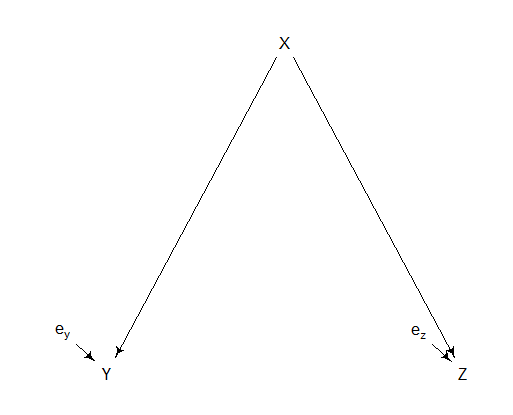
\includegraphics[width=5cm]{scenario1.DAG.png}
\centering
\end{figure}


In this first case, Y is not related to Z.
The second scenario would be:

\begin{lstlisting}
scenario2.DAG <- dagitty("dag {
X -> Y
X -> Z
Y -> Z
e_y -> Y
e_z -> Z
}")

coordinates(scenario2.DAG) <- list(x = c(Y = 1, X = 2, Z = 3, e_y = 0.75, e_z = 2.75), y = c(Y = 3, X = 1, Z = 3, e_y = 2.75, e_z = 2.75))
drawdag(scenario2.DAG)

\end{lstlisting}

\begin{figure}[h]
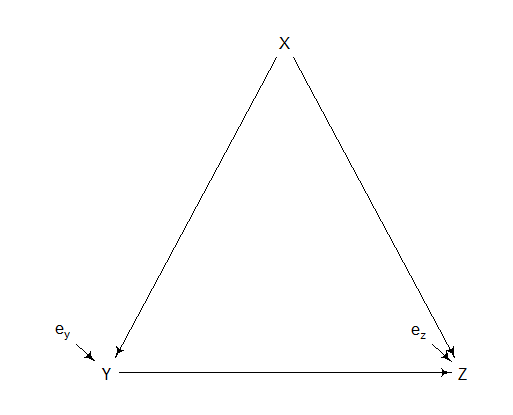
\includegraphics[width=5cm]{scenario2.DAG.png}
\centering
\end{figure}


In this second case, Y does have an effect over Z.
It is important to tell the difference between both of them, as the correct model to apply will be different. How can we tell if our data corresponds to one scenario or another? We have created the following function to do so:

 

\section{What to do when there is a common effect}

\section{Complex cases and backdoor criteria}

\section{Conclusion}

\section{References}

\end{document}